%!TEX root = ../document.tex
\chapter{Empirical settings and methods}
In this chapter...

\section{Empirical setting}
The collection of data material used in this thesis took part in late autumn 2013, at a high school located in the center of Oslo. The school has a high limit for admission, with a lower requirement of 43.5 points out of 60 in 2010 \citep{utdanningsetaten}. Thus, the students at this school are mostly high achievers. 

Contact with the school was first initiated through Intermedia, and a presentational flier was sent as an explanation of the project (insert an appendix ref here). Luckily our request coincided perfectly with a two-week time frame for reviewing photosynthesis in one of the teacher's biology classes.\sout{He was therefore willing to swap out the experiment described in the textbook with an experiment using our application.} He was therefore willing to use our application instead of performing the experiments described in the textbook. 

The class selected for the experiment was a biology class at the highest level offered at the school, biology 2, which has an extensive curriculum covering e.g photosynthesis, enzymes and energy transmitters (insert ref to photosynthesis chapter). The students were between 17 and 18 years of age, and for the main part of our data collection most of the 20 students were present. All the students agreed to participate in the study, but due to technical limitations and a busy time schedule, most of the data collection was only done with a small sample of the group. 

\subsection{Experiment}
\subsubsection{Planning}
An initial planning and presentational meeting was held on the 21st. of October with the teacher at Foss VGS. A thorough presentation and demonstration of the system was given, along with a discussion of the functionalities of the system, to see if it would spark some ideas for experiments. 

Stressing the importance of a scientific method, the teacher suggested that we could conduct two experiments, using the different sensors in the system to change one variable, while keeping the others relatively controlled. We agreed that the factor which would be easiest to control, yet yield interesting results was light intensity and light quality (wavelength). The first experiment would then involve keeping the plant located in a window facing west, receiving sunlight and light from the fluorescent indoor-lighting. While we in the second experiment would relocate the plant to a (presumably) light proof cabinet, where it would only receive light of a known wavelength. Each of the two experiments would have a duration of approximately one week depending on the time needed for usable results. 

\subsubsection{The experiments}
The project was presented and the first experiment initiated on Friday 25th of October. This went on for seven days until Friday 1st of November when the second experiment was initiated. The second experiment went on for 13 days until Wednesday 13th of November when the primary data collection session took place. During the experiments we were present at four separate occasions, observing what the teacher was focusing on, and which parts of the photosynthesis the students found most difficult. In addition we were answering questions about the system, and observed how the system was used by the teacher and how the students related to it. 

\subsubsection*{The plant in the window}
The first experiment was conducted with a setup in the window as shown in figure~\ref{fig:windowplant}. The system was located in the front of the classroom near a door leading to the adjacent classroom, this meant it was visible and in reach of everyone walking by. The system was in the windowsill and there was a radiator located on the wall just beneath the plant. As figure~\ref{fig:windowsystemplant} shows, there is between 50 and 70 seeds in the pot. The plant was exposed to sunlight or daylight depending on the weather, but it was also exposed to the fluorescent indoor-lighting in the ceiling. Due to the time of year, and lack of people using the classroom in the evening, this meant that the plant would get light in the period between 08:00 17:00.

It turned out that the system was draining power from a power outlet that was either connected to the light, or timer based, since the system went down and did not post data between 19:00 and 07:00. We did also have some technical issues with the system the weekend from 25th of October to 27th of October, meaning that we missed data from the first seeds germinating.

\begin{figure}
\centering
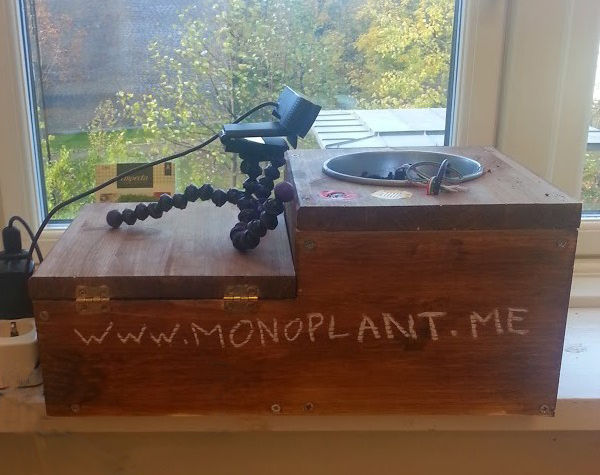
\includegraphics[width=0.8\textwidth]{img/empiricalsetting/window.jpg}
\caption{The system located in the window}
\label{fig:windowplant}
\end{figure}

\begin{figure}
\centering
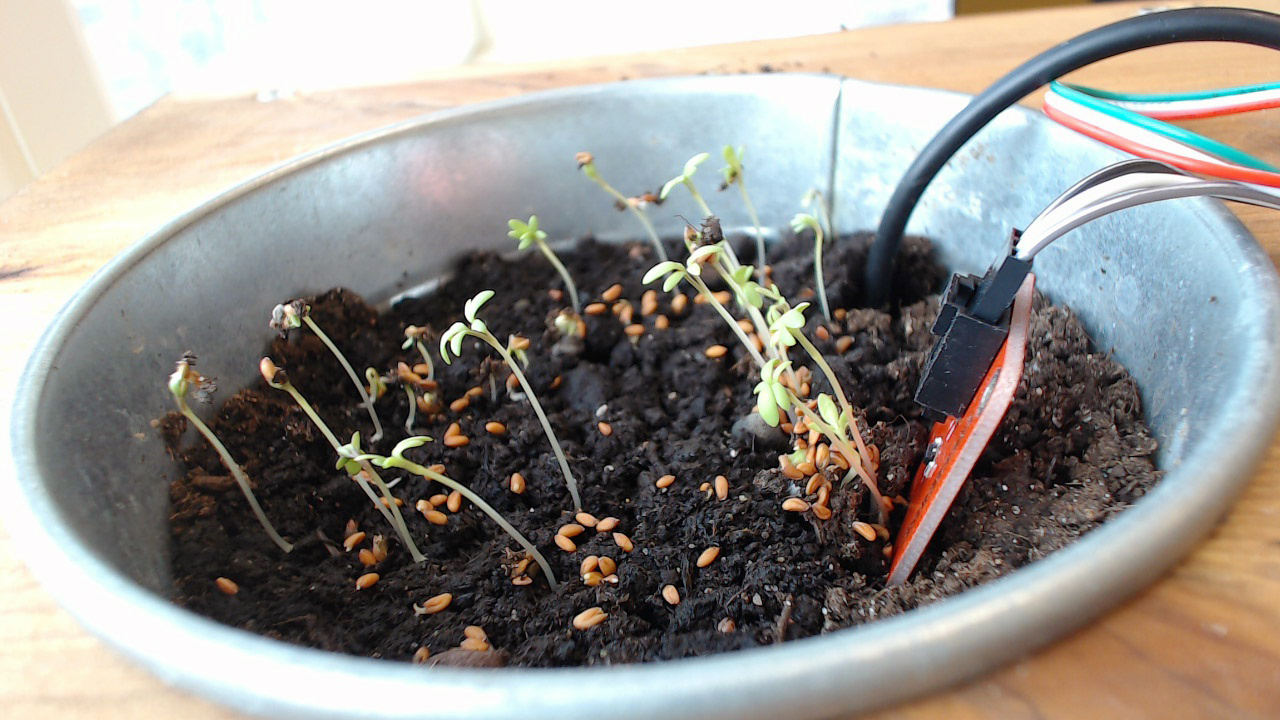
\includegraphics[width=0.8\textwidth]{img/empiricalsetting/windowsystem.jpg}
\caption{The plant receiving natural light}
\label{fig:windowsystemplant}
\end{figure}



\subsubsection*{The plant in the cabinet}
The second experiment was conducted with a setup in a cabinet as shown in figure~\ref{fig:cabinetplant}. The cabinet was located in a corner in the front of the classroom behind the teachers desk, this meant that the plant was hidden and not nearly as accessible as the plant in the window. The picture in figure~\ref{fig:cabinetplant} is taken with flash and light from the room coming in to the cabinet, hence it does not reflect the lighting conditions in the cabinet during the experiment. The cabinet door was closed and the lamp above the plant was emitting green light 24 hours a day, hence figure~\ref{fig:cabinetsystemplant} shows the lighting conditions better. It is also worth noting that the pot contains between 100 and 120 seeds. When this experiment took place we did not have any technical issues, the system posted data continuously for the whole period.

\begin{figure}
\centering
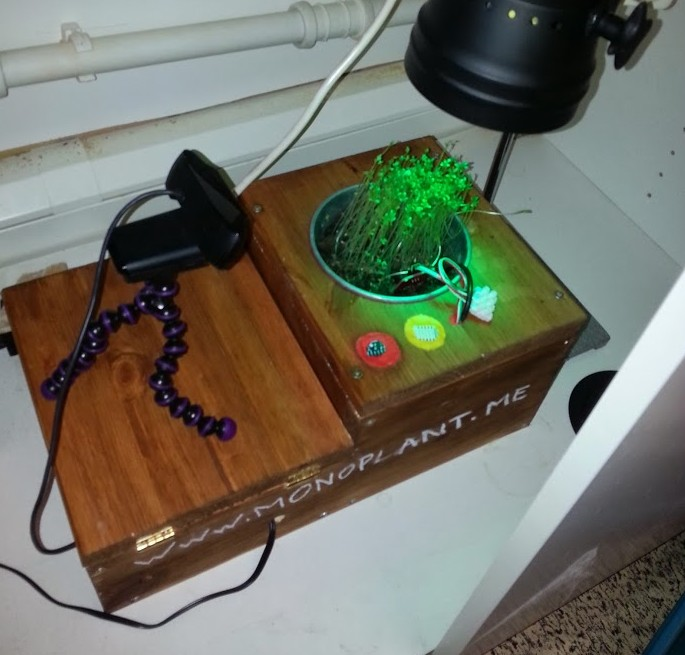
\includegraphics[width=0.8\textwidth]{img/empiricalsetting/cupboard.jpg}
\caption{The system located in the cabinet}
\label{fig:cabinetplant}
\end{figure}

\begin{figure}
\centering
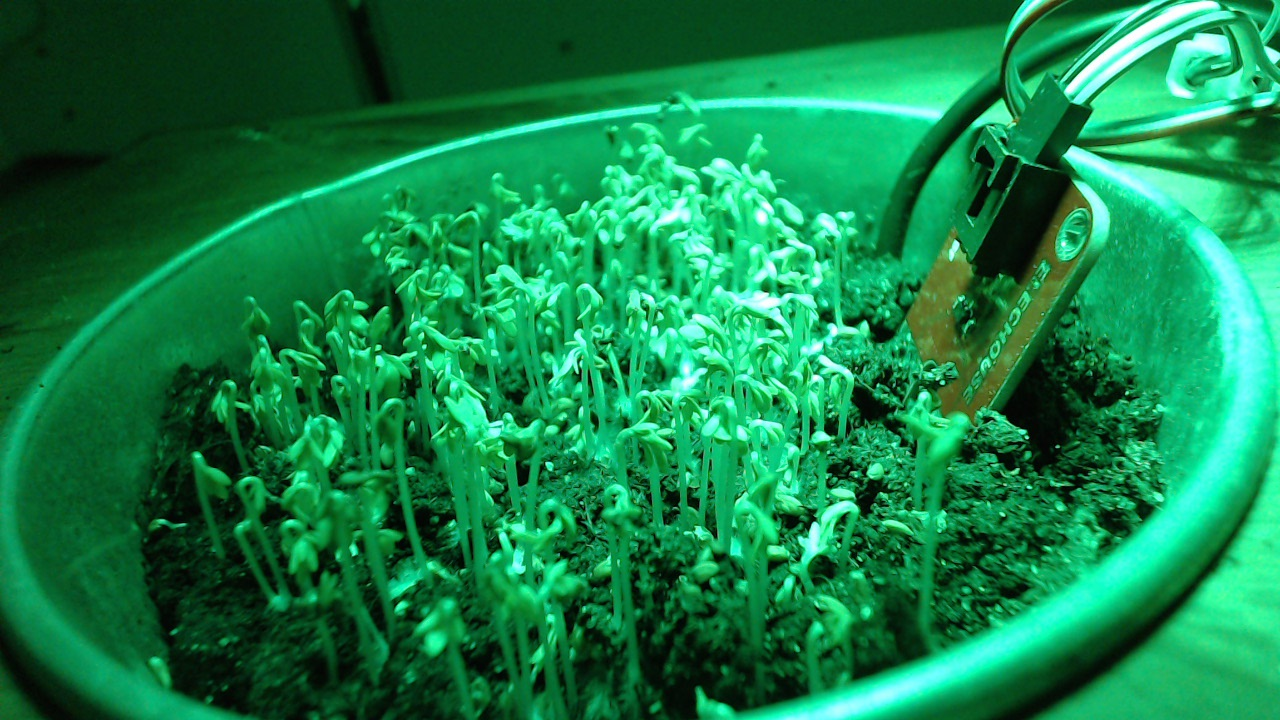
\includegraphics[width=0.8\textwidth]{img/empiricalsetting/cupboardsystem.jpg}
\caption{The plant in the cabinet, receiving green light}
\label{fig:cabinetsystemplant}
\end{figure}


\subsection{Methods}
Different methods for data collection was discussed and reviewed early on in the project. Our most influential source, regarding both paradigm, methodology and method was the tradition for using qualitative data in information systems research at department of informatics. As our primary data source we chose video data with the use of multiple cameras and a screen-dump. This was collected during a 45-minute session after the completion of the experiments, resulting in 3x45 minutes of video data and 45 minutes of audio data. Supplementary data from this session includes the written answers from the groups which were not filmed, and our personal notes of general observations. \sout{In addition to this we were present at five occasions preceding the session, taking notes.} In the following sections the methods used will be discussed. 

\subsubsection{Video and audio}
It was determined early in the project that video and audio recording were to be used. Perhaps the primary reason for this was the tradition at Intermedia, as video data collection has been used and thoroughly tested by a number of researchers here. This meant that we would get a lot of help from co-located researchers in what microphones to use, placement of cameras, operation of the equipment, etc. 

A total of 45 minutes of video and audio was recorded, using three separate video sources, and three microphones. One camera was placed in front of the group, able to capture facial expressions and where the students were looking. This camera had an external microphone connected which we placed on the table in front of the students, allowing us to filter out some of the noise in the classroom and making the voices of the students clearer. The second camera was placed behind the students on their right hand side, facing the computer screen. This camera's primary function was to capture where the students were pointing and what they where doing on the laptop. The audio source from the second camera was the built-in microphone, which proved to cover most of the noise from the whole classroom. In addition to the video cameras we recorded a screen capture from the laptop, showing exactly what the students were doing in the system. The laptop had a built-in microphone as well but we only used the sound from camera two and the laptop to synchronize the different videos.
\begin{figure}
\centering
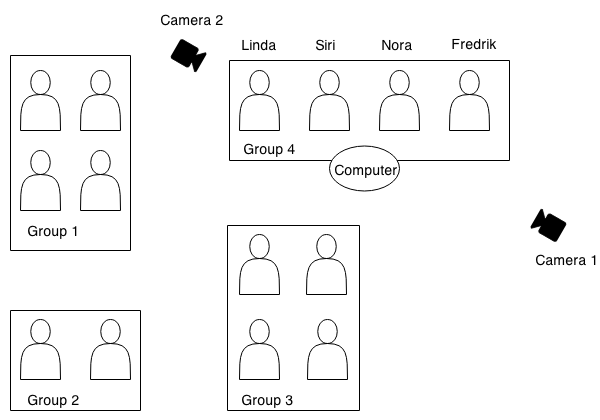
\includegraphics[width=0.8\textwidth]{img/empiricalsetting/class_diagram.png}
\caption{Camera setup}
\label{fig:camerasetup}
\end{figure}

\subsubsection{Passive observation}
During the experiments we were present at four separate occasions. The primary reason was to ensure that the system was working, assist with any technical difficulties regarding the user interface, and to ensure a smooth operation of the experiments. But we would also take notes regarding how the system was used in the education, if or how students showed interest in the experiments, and how the teacher was conveying information about photosynthesis in general. While these observation sessions were not thoroughly planned, and the data material never systematized, it proved to be a good supplementary data source to help us structure and make sense of our primary data. We would later on also use these notes as discussion points when reviewing the data material. 

\subsubsection{Student produced material}

\subsubsection{Web logs}
In order to review activity on the web page (\url{http://monoplant.me}), Google Analytics tracking system was installed. Although we did not use this extensively, it allowed us to see if and how often the system was used, and if students were using it at home or only during classes. 

\subsection{Analytical Procedures}
\subsubsection{Interaction analysis}
%Crang & cook: Video recordings can be criticized by pointing out that it is the researcher that selects the frame and focus. Hence the data can become biased. However, by trying to frame interaction generically, and providing a video, getting other people to double check coding and transcription.
The analytical procedure employed within this thesis is \emph{Interaction analysis} \citep{jordan1995interaction}, which emerged from fields such as ethnography, sociolinguistics, ethnomethodology, conversation analysis, and sociocultural theories. \citeauthor{jordan1995interaction} describes it as follows:

\begin{quote}
An interdisciplinary method for the empirical investigation of the interaction of human
beings with each other and with objects in their environment. It investigates human
activities such as talk, nonverbal interaction, and the use of artifacts and technologies,
identifying routine practices and problems and the resources for their solution \citep[p39]{jordan1995interaction}
\end{quote}

For Interaction analysis to become a reality video and audio recording technology has been a vital resource. The combination of recording talk as well as nonverbal interaction and the ability to replay a sequence as many times as necessary gives us the possibility to analyze more thoroughly. Combining this micro-level data of interaction with ethnographic data gives us a means of analyzing how the interaction is part of the situated context and institutional practices. \citep{furberg2009scientific}. 

\sout{Even though we have done a case study in a real educational setting, considering these ethnographic data is important if we are to keep a dialogic perspective.}


\subsubsection{Making sense of the data}
\citeauthor{derry2010conducting} speaks about two different approaches to select parts of a video corpus for further examination. These two are the \emph{inductive} approach and the \emph{deductive} approach. Inductive approaches apply when a minimally edited video corpus is collected and investigated with broad questions in mind but without a strong orienting theory. Deductive approaches involve identifying or creating a suitable video corpus and systematically sampling from it to examine specific re-search questions. \citep{derry2010conducting} To start with, we clearly fit into the inductive approach, but as every researcher experiences, once you find something you start looking for it, hence our approach became leaned more to the deductive side later in our analysis.

To make sense of the data gathered we looked at it in several different ways with different focuses. Below is a chronological list of the ways we approached the data. 


\begin{enumerate}
\item{Initial screening of main video corpus, locating interesting interaction}
\item{Transcription of main video corpus}
\item{Watching additional video material to make detailed notes on interactions with the system}
\item{Watching the main video corpus with our supervisor and discussing which events and interactions are interesting and/or can be linked to existing theory}
\item{Detailed transcriptions of the most interesting interactions}
\item{Writing explanations of these interactions}
\item{Linking interactions to support each other}
\item{Cut excerpts that did not fit together with other excerpts}
\item{Linking chunks of interactions to related theory}
\end{enumerate}

As shown in the list, our approach was open to begin with, but became more and more narrowed down once we found interesting interaction. 


\subsection{Ethics}
Prior to the data collection, an application was sent to NSD (Norwegian Social Science Data Services) requesting permission to film the students. The application was approved with only minor changes to how the material was to be treated after completion. In addition all the students taking the class was given an agreement form, stating that participation was voluntary, and that all material would be kept anonymous (see appendix). 

Throughout this thesis, and in the transcript of video data, all the students names have been replaced by pseudonyms. The data material containing identifying information of the students has been and will be stored securely on a separate hard drive at Intermedia, and will be deleted in October 2014. 

During our time at Foss VGS we were always open about our role as researchers, and explained on several occations how the data was going to be used. 




